\documentclass[
  jou,
  floatsintext,
  longtable,
  nolmodern,
  notxfonts,
  notimes,
  colorlinks=true,linkcolor=blue,citecolor=blue,urlcolor=blue]{apa7}

\usepackage{amsmath}
\usepackage{amssymb}



\usepackage[bidi=default]{babel}
\babelprovide[main,import]{english}


% get rid of language-specific shorthands (see #6817):
\let\LanguageShortHands\languageshorthands
\def\languageshorthands#1{}

\RequirePackage{longtable}
\RequirePackage{threeparttablex}

\makeatletter
\renewcommand{\paragraph}{\@startsection{paragraph}{4}{\parindent}%
	{0\baselineskip \@plus 0.2ex \@minus 0.2ex}%
	{-.5em}%
	{\normalfont\normalsize\bfseries\typesectitle}}

\renewcommand{\subparagraph}[1]{\@startsection{subparagraph}{5}{0.5em}%
	{0\baselineskip \@plus 0.2ex \@minus 0.2ex}%
	{-\z@\relax}%
	{\normalfont\normalsize\bfseries\itshape\hspace{\parindent}{#1}\textit{\addperi}}{\relax}}
\makeatother




\usepackage{longtable, booktabs, multirow, multicol, colortbl, hhline, caption, array, float, xpatch}
\setcounter{topnumber}{2}
\setcounter{bottomnumber}{2}
\setcounter{totalnumber}{4}
\renewcommand{\topfraction}{0.85}
\renewcommand{\bottomfraction}{0.85}
\renewcommand{\textfraction}{0.15}
\renewcommand{\floatpagefraction}{0.7}

\usepackage{tcolorbox}
\tcbuselibrary{listings,theorems, breakable, skins}
\usepackage{fontawesome5}

\definecolor{quarto-callout-color}{HTML}{909090}
\definecolor{quarto-callout-note-color}{HTML}{0758E5}
\definecolor{quarto-callout-important-color}{HTML}{CC1914}
\definecolor{quarto-callout-warning-color}{HTML}{EB9113}
\definecolor{quarto-callout-tip-color}{HTML}{00A047}
\definecolor{quarto-callout-caution-color}{HTML}{FC5300}
\definecolor{quarto-callout-color-frame}{HTML}{ACACAC}
\definecolor{quarto-callout-note-color-frame}{HTML}{4582EC}
\definecolor{quarto-callout-important-color-frame}{HTML}{D9534F}
\definecolor{quarto-callout-warning-color-frame}{HTML}{F0AD4E}
\definecolor{quarto-callout-tip-color-frame}{HTML}{02B875}
\definecolor{quarto-callout-caution-color-frame}{HTML}{FD7E14}

\newlength\Oldarrayrulewidth
\newlength\Oldtabcolsep


\usepackage{hyperref}




\providecommand{\tightlist}{%
  \setlength{\itemsep}{0pt}\setlength{\parskip}{0pt}}
\usepackage{longtable,booktabs,array}
\usepackage{calc} % for calculating minipage widths
% Correct order of tables after \paragraph or \subparagraph
\usepackage{etoolbox}
\makeatletter
\patchcmd\longtable{\par}{\if@noskipsec\mbox{}\fi\par}{}{}
\makeatother
% Allow footnotes in longtable head/foot
\IfFileExists{footnotehyper.sty}{\usepackage{footnotehyper}}{\usepackage{footnote}}
\makesavenoteenv{longtable}

\usepackage{graphicx}
\makeatletter
\def\maxwidth{\ifdim\Gin@nat@width>\linewidth\linewidth\else\Gin@nat@width\fi}
\def\maxheight{\ifdim\Gin@nat@height>\textheight\textheight\else\Gin@nat@height\fi}
\makeatother
% Scale images if necessary, so that they will not overflow the page
% margins by default, and it is still possible to overwrite the defaults
% using explicit options in \includegraphics[width, height, ...]{}
\setkeys{Gin}{width=\maxwidth,height=\maxheight,keepaspectratio}
% Set default figure placement to htbp
\makeatletter
\def\fps@figure{htbp}
\makeatother


% definitions for citeproc citations
\NewDocumentCommand\citeproctext{}{}
\NewDocumentCommand\citeproc{mm}{%
  \begingroup\def\citeproctext{#2}\cite{#1}\endgroup}
\makeatletter
 % allow citations to break across lines
 \let\@cite@ofmt\@firstofone
 % avoid brackets around text for \cite:
 \def\@biblabel#1{}
 \def\@cite#1#2{{#1\if@tempswa , #2\fi}}
\makeatother
\newlength{\cslhangindent}
\setlength{\cslhangindent}{1.5em}
\newlength{\csllabelwidth}
\setlength{\csllabelwidth}{3em}
\newenvironment{CSLReferences}[2] % #1 hanging-indent, #2 entry-spacing
 {\begin{list}{}{%
  \setlength{\itemindent}{0pt}
  \setlength{\leftmargin}{0pt}
  \setlength{\parsep}{0pt}
  % turn on hanging indent if param 1 is 1
  \ifodd #1
   \setlength{\leftmargin}{\cslhangindent}
   \setlength{\itemindent}{-1\cslhangindent}
  \fi
  % set entry spacing
  \setlength{\itemsep}{#2\baselineskip}}}
 {\end{list}}
\usepackage{calc}
\newcommand{\CSLBlock}[1]{\hfill\break\parbox[t]{\linewidth}{\strut\ignorespaces#1\strut}}
\newcommand{\CSLLeftMargin}[1]{\parbox[t]{\csllabelwidth}{\strut#1\strut}}
\newcommand{\CSLRightInline}[1]{\parbox[t]{\linewidth - \csllabelwidth}{\strut#1\strut}}
\newcommand{\CSLIndent}[1]{\hspace{\cslhangindent}#1}





\usepackage{newtx}

\defaultfontfeatures{Scale=MatchLowercase}
\defaultfontfeatures[\rmfamily]{Ligatures=TeX,Scale=1}





\title{Using Quarto to Generate Documents in APA Style (7th Edition)}


\shorttitle{Template for the apaquarto Extension}


\usepackage{etoolbox}









\authorsnames[{1},{1},{2,3},{4}]{Ana Fulano,Blanca Zutano,Carina
Mengano,Dolorita C. Perengano}







\authorsaffiliations{
{Department of Psychology, Ana and Blanca's University},{Carina's
Primary Affiliation},{Carina's Secondary Affiliation},{Buffalo, NY }}




\leftheader{Fulano, Zutano, Mengano and C.}



\abstract{This document is a template demonstrating the apaquarto
format.}

\keywords{keyword1, keyword2, keyword3}

\authornote{\par{\addORCIDlink{Ana
Fulano}{0000-0000-0000-0001}}\par{\addORCIDlink{Blanca
Zutano}{0000-0000-0000-0002}}\par{\addORCIDlink{Carina
Mengano}{0000-0000-0000-0003}}\par{\addORCIDlink{Dolorita C.
Perengano}{0000-0000-0000-0004}} 
\par{Carina Mengano is now at Generic University. }
\par{   The authors have no conflicts of interest to
disclose.    Author roles were classified using the Contributor Role Taxonomy (CRediT; https://credit.niso.org/) as follows: Ana
Fulano:   conceptualization, writing; Blanca Zutano:   project
administration, formal analysis; Carina Mengano:   formal
analysis, writing; Dolorita C. Perengano:   writing, methodology, formal
analysis}
\par{Correspondence concerning this article should be addressed to Ana
Fulano, Department of Psychology, Ana and Blanca's University, 1234
Capital St., Albany, NY 12084-1234, USA, Email: sm@example.org}
}

\usepackage{pbalance} 
\usepackage{float}
\makeatletter
\let\oldtpt\ThreePartTable
\let\endoldtpt\endThreePartTable
\def\ThreePartTable{\@ifnextchar[\ThreePartTable@i \ThreePartTable@ii}
\def\ThreePartTable@i[#1]{\begin{figure}[!htbp]
\onecolumn
\begin{minipage}{0.5\textwidth}
\oldtpt[#1]
}
\def\ThreePartTable@ii{\begin{figure}[!htbp]
\onecolumn
\begin{minipage}{0.5\textwidth}
\oldtpt
}
\def\endThreePartTable{
\endoldtpt
\end{minipage}
\twocolumn
\end{figure}}
\makeatother


\makeatletter
\let\endoldlt\endlongtable		
\def\endlongtable{
\hline
\endoldlt}
\makeatother

\newenvironment{twocolumntable}% environment name
{% begin code
\begin{table*}[!htbp]%
\onecolumn%
}%
{%
\twocolumn%
\end{table*}%
}% end code

\urlstyle{same}



\makeatletter
\@ifpackageloaded{caption}{}{\usepackage{caption}}
\AtBeginDocument{%
\ifdefined\contentsname
  \renewcommand*\contentsname{Table of contents}
\else
  \newcommand\contentsname{Table of contents}
\fi
\ifdefined\listfigurename
  \renewcommand*\listfigurename{List of Figures}
\else
  \newcommand\listfigurename{List of Figures}
\fi
\ifdefined\listtablename
  \renewcommand*\listtablename{List of Tables}
\else
  \newcommand\listtablename{List of Tables}
\fi
\ifdefined\figurename
  \renewcommand*\figurename{Figure}
\else
  \newcommand\figurename{Figure}
\fi
\ifdefined\tablename
  \renewcommand*\tablename{Table}
\else
  \newcommand\tablename{Table}
\fi
}
\@ifpackageloaded{float}{}{\usepackage{float}}
\floatstyle{ruled}
\@ifundefined{c@chapter}{\newfloat{codelisting}{h}{lop}}{\newfloat{codelisting}{h}{lop}[chapter]}
\floatname{codelisting}{Listing}
\newcommand*\listoflistings{\listof{codelisting}{List of Listings}}
\makeatother
\makeatletter
\makeatother
\makeatletter
\@ifpackageloaded{caption}{}{\usepackage{caption}}
\@ifpackageloaded{subcaption}{}{\usepackage{subcaption}}
\makeatother

% From https://tex.stackexchange.com/a/645996/211326
%%% apa7 doesn't want to add appendix section titles in the toc
%%% let's make it do it
\makeatletter
\xpatchcmd{\appendix}
  {\par}
  {\addcontentsline{toc}{section}{\@currentlabelname}\par}
  {}{}
\makeatother

\begin{document}

\maketitle


\setcounter{secnumdepth}{-\maxdimen} % remove section numbering

\setlength\LTleft{0pt}


This is my introductory paragraph. The title will be placed above it
automatically. \emph{Do not start with an introductory heading} (e.g.,
``Introduction''). The title acts as your Level 1 heading for the
introduction.

Details about writing headings with markdown in APA style are
\href{https://wjschne.github.io/apaquarto/writing.html\#headings-in-apa-style}{here}.

\subsection{Displaying Figures}\label{displaying-figures}

A reference label for a figure must have the prefix \texttt{fig-}, and
in a code chunk, the caption must be set with \texttt{fig-cap}. Captions
are in
\href{https://apastyle.apa.org/style-grammar-guidelines/capitalization/title-case}{title
case}.

\begin{figure}[!htbp]

{\caption{{The Figure Caption}{\label{fig-myplot}}}}

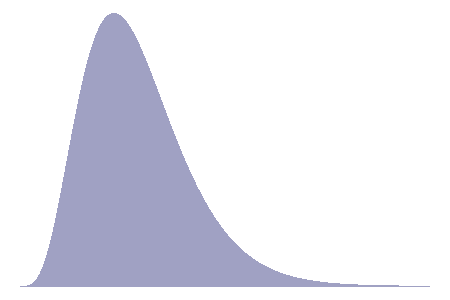
\includegraphics{example_files/figure-pdf/fig-myplot-1.pdf}

{\noindent \emph{Note.} This is the note below the figure.}

\end{figure}

To refer to any figure or table, use the \texttt{@} symbol followed by
the reference label (e.g., Figure~\ref{fig-myplot}).

\subsection{Imported Graphics}\label{imported-graphics}

One way to import an existing graphic as a figure is to use
\texttt{knitr::include\_graphics} in a code chunk. For example,
Figure~\ref{fig-import1} is an imported image. Note that in
apaquarto-pdf documents, we can specify that that a figure or table
should span both columns when in journal mode by setting the
\texttt{apa-twocolumn} chunk option to \texttt{true}. For other formats,
this distinction does not matter.

\begin{figure}[!htbp]

{\caption{{An Imported Graphic}{\label{fig-import1}}}}

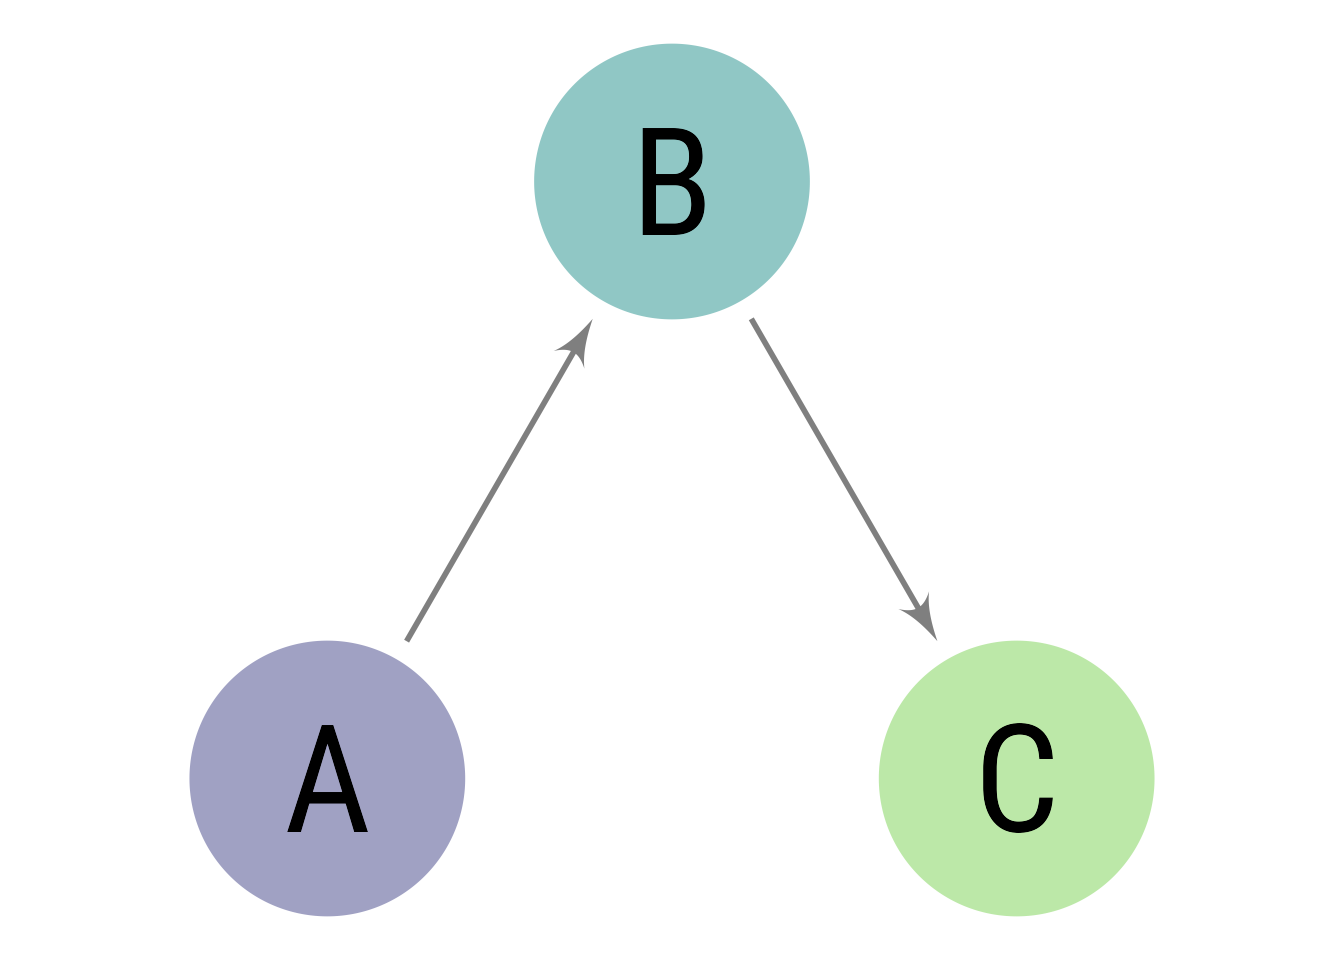
\includegraphics[width=0.48\textwidth,height=\textheight]{sampleimage.png}

{\noindent \emph{Note.} A note below the figure}

\end{figure}

Figure graphics can be imported directly with Markdown, as with
Figure~\ref{fig-import2}.

\begin{figure}[!htbp]

{\caption{{Another Way to Import Graphics}{\label{fig-import2}}}}

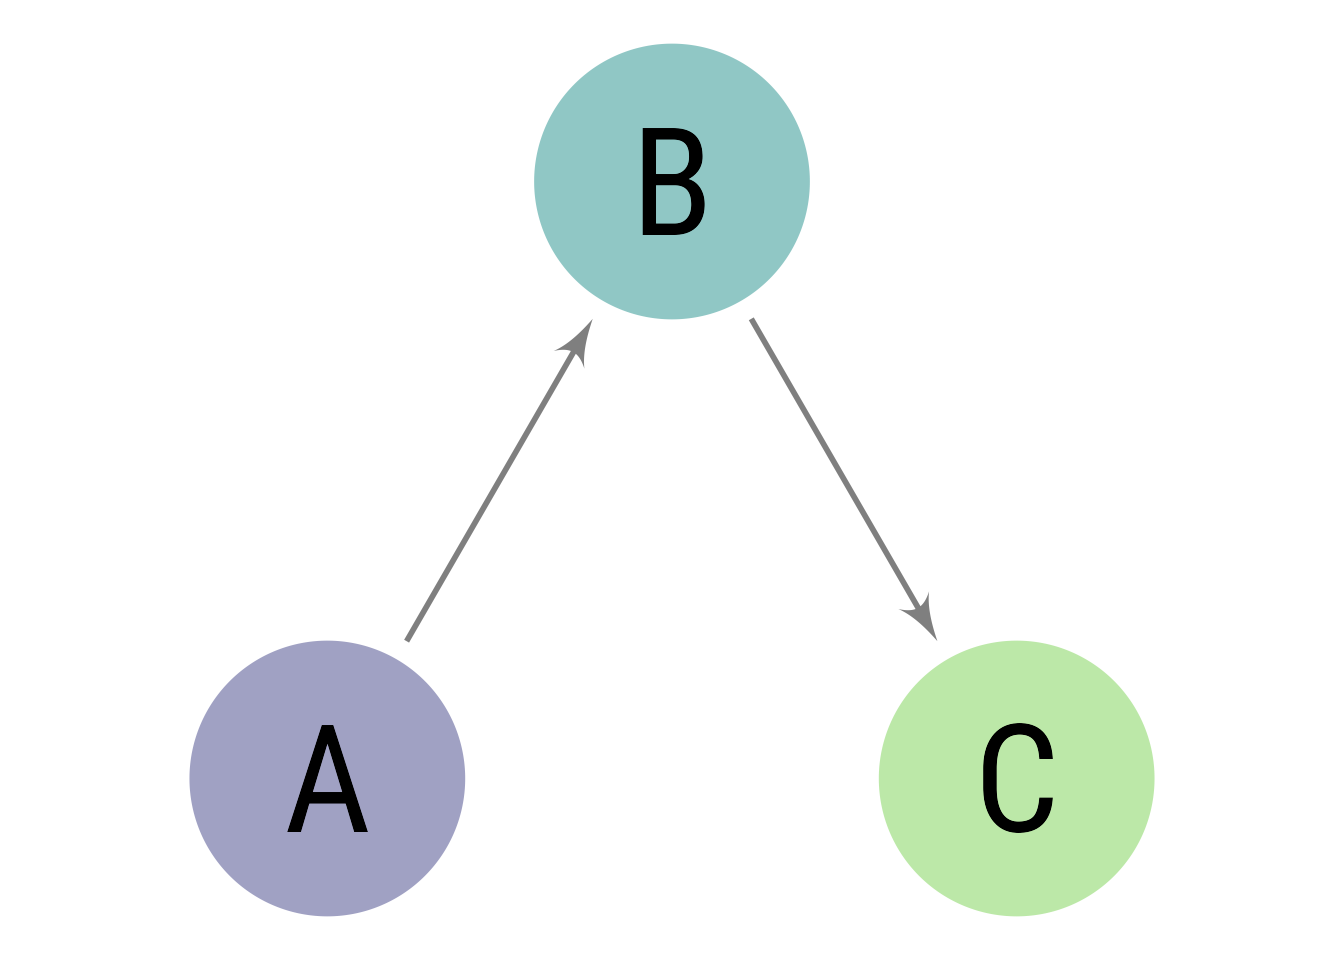
\includegraphics[width=0.49\textwidth,height=\textheight]{sampleimage.png}

{\noindent \emph{Note.} A note below the figure}

\end{figure}

Which style of creating figures you choose depends on preference and
need.

\subsection{Displaying Tables}\label{displaying-tables}

We can make a table the same way as a figure. Generating a table that
conforms to APA format in all document formats can be tricky. When the
table is simple, the \texttt{kable} function from knitr works well. Feel
free to experiment with different methods, but I have found that David
Gohel's \href{https://davidgohel.github.io/flextable/}{flextable} to be
the best option when I need something more complex.

\begin{ThreePartTable}

\begin{longtable}[]{@{}rl@{}}

\caption{\label{tbl-mytable}The Table Caption}

\tabularnewline

\toprule\noalign{}
Numbers & Letters \\
\midrule\noalign{}
\endhead
\bottomrule\noalign{}
\endlastfoot
1 & A \\
2 & B \\
3 & C \\
4 & D \\

\end{longtable}

{\noindent \emph{Note.} The note below the table.}

\end{ThreePartTable}

To refer to this table in text, use the \texttt{@} symbol followed by
the reference label like so: As seen in Table~\ref{tbl-mytable}, the
first few numbers and letters of the alphabet are displayed.

In Table~\ref{tbl-mymarkdowntable}, there is an example of a plain
markdown table with a note below it.

\begin{ThreePartTable}

\begin{longtable}[]{@{}llrc@{}}
\caption{Table Caption of a Markdown
Table}\label{tbl-mymarkdowntable}\tabularnewline
\toprule\noalign{}
Default & Left & Right & Center \\
\midrule\noalign{}
\endfirsthead
\toprule\noalign{}
Default & Left & Right & Center \\
\midrule\noalign{}
\endhead
\bottomrule\noalign{}
\endlastfoot
12 & 12 & 12 & 12 \\
123 & 123 & 123 & 123 \\
1 & 1 & 1 & 1 \\
\end{longtable}

{\noindent \emph{Note.} This is a note below the markdown table.}

\end{ThreePartTable}

In \{tbl-mymarkdowntable2\}, there are some numbers.

\begin{longtable}[]{@{}llrc@{}}
\toprule\noalign{}
Default & Left & Right & Center \\
\midrule\noalign{}
\endhead
\bottomrule\noalign{}
\endlastfoot
12 & 12 & 12 & 12 \\
123 & 123 & 123 & 123 \\
1 & 1 & 1 & 1 \\
\end{longtable}

What if you want the tables and figures to be at the end of the
document? In the .pdf format, you can set the \texttt{floatsintext}
option to false. For .html and .docx documents, there is not yet an
automatic way to put tables and figures at the end. You can, of course,
just put them all at the end, in order. The reference labels will work
no matter where they are in the text.

\subsection{Tables and Figures Spanning Two Columns in Journal
Mode}\label{tables-and-figures-spanning-two-columns-in-journal-mode}

When creating tables and figures in journal mode, care must be taken not
to make figures and tables wider than the columns, otherwise \LaTeX
sometimes makes them disappear.

As demonstrated in Figure~\ref{fig-twocolumn}, you can make figures
tables span the two columns by setting the \texttt{apa-twocolumn} chunk
option to \texttt{true}.

\begin{figure*}[!htbp]

{\caption{{A Figure Spanning Two Columns When in Journal
Mode}{\label{fig-twocolumn}}}}

\begin{center}
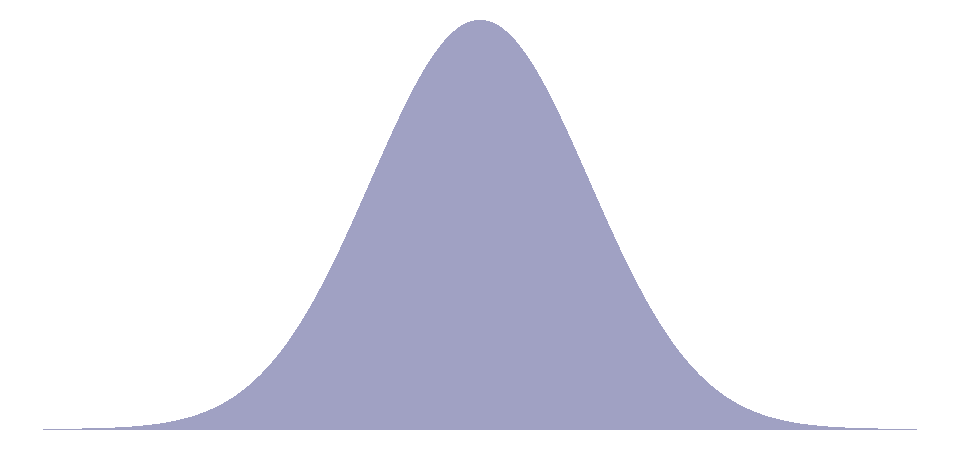
\includegraphics{example_files/figure-pdf/fig-twocolumn-1.pdf}
\end{center}

{\noindent \emph{Note.} Figures in two-column mode are only different
for jou mode in .pdf documents}

\end{figure*}

\subsection{Math and Equations}\label{math-and-equations}

Inline math uses \LaTeX syntax with single dollar signs. For example,
the reliability coefficient of my measure is \(r_{XX}=.95\).

If you want to display and refer to a specific formula, enclose the
formula in two dollar signs. After the second pair of dollar signs,
place the label in curly braces. The label should have an \texttt{\#eq-}
prefix. To refer to the formula, use the same label but with the
\texttt{@} symbol. For example, Equation~\ref{eq-euler} is Euler's
Identity, which is much admired for its elegance.

\subsection{Citations}\label{citations}

See
\href{https://quarto.org/docs/authoring/footnotes-and-citations.html}{here}
for instructions on setting up citations and references.

A parenthetical citation requires square brackets
(\citeproc{ref-CameronTrivedi2013}{Cameron \& Trivedi, 2013}). This
reference was in my bibliography file. An in-text citation is done like
so:

Cameron and Trivedi (\citeproc{ref-CameronTrivedi2013}{2013}) make some
important points \ldots{}

See
\href{https://wjschne.github.io/apaquarto/writing.html\#references}{here}
for explanations, examples, and citation features exclusive to
apaquarto. For example, apaquarto can automatically handle possessive
citations:

Schneider and McGrew's (\citeproc{ref-schneider2012cattell}{2012})
position was \ldots{}

\subsection{Masking Author Identity for Peer
Review}\label{masking-author-identity-for-peer-review}

Setting \texttt{mask} to \texttt{true} will remove author names,
affiliations, and correspondence from the title page. Any references
listed in the \texttt{masked-citations} field will be masked as well.
See
\href{https://wjschne.github.io/apaquarto/writing.html\#masked-citations-for-anonymous-peer-review}{here}
for more information.

\begin{equation}\phantomsection\label{eq-euler}{
e^{i\pi}+1=0
}\end{equation}

\subsection{Block Quotes}\label{block-quotes}

Sometimes you want to give a longer quote that needs to go in its own
paragraph. Block quotes are on their own line starting with the
\textgreater{} character. For example, Austen's
(\citeproc{ref-austenMansfieldPark1990}{1814/1990}) \emph{Mansfield
Park} has some memorable insights about the mind:

\begin{quote}
If any one faculty of our nature may be called more wonderful than the
rest, I do think it is memory. There seems something more speakingly
incomprehensible in the powers, the failures, the inequalities of
memory, than in any other of our intelligences. The memory is sometimes
so retentive, so serviceable, so obedient; at others, so bewildered and
so weak; and at others again, so tyrannic, so beyond control! We are, to
be sure, a miracle every way; but our powers of recollecting and of
forgetting do seem peculiarly past finding out. (p.~163)
\end{quote}

If your quote has multiple paragraphs, like this passage from Brown
(\citeproc{ref-brownHowKilledPluto2012}{2012}), separate them with a
lone \texttt{\textgreater{}} character between the lines:

\begin{quote}
In the entire field of astronomy, there is no word other than
\emph{planet} that has a precise, lawyerly definition, in which certain
criteria are specifically enumerated. Why does \emph{planet} have such a
definition but \emph{star}, \emph{galaxy}, and \emph{giant molecular
cloud} do not? Because in astronomy, as in most sciences, scientists
work by concepts rather than by definitions. The concept of a star is
clear; a star is a collection of gas with fusion reactions in the
interior giving off energy. A galaxy is a large, bound collection of
stars. A giant molecular cloud is a giant cloud of molecules. The
concept of a planet---in the eight-planet solar system---is equally
simple to state. A planet is a one of a small number of bodies that
dominate a planetary system. That is a concept, not a definition. How
would you write that down in a precise definition?

I wouldn't. Once you write down a definition with lawyerly precision,
you get the lawyers involved in deciding whether or not your objects are
planets. Astronomers work in concepts. We rarely call in the attorneys
for adjudication. (p.~242)
\end{quote}

\subsection{Hypotheses, Aims, and
Objectives}\label{hypotheses-aims-and-objectives}

The last paragraph of the introduction usually states the specific
hypotheses of the study, often in a way that links them to the research
design.

\section{Method}\label{method}

General remarks on method. This paragraph is optional.

Not all papers require each of these sections. Edit them as needed.
Consult the \href{https://apastyle.apa.org/jars}{Journal Article
Reporting Standards} for what is needed for your type of article.

\subsection{Participants}\label{participants}

Who are they? How were they recruited? Report criteria for participant
inclusion and exclusion. Perhaps some basic demographic stats are in
order. A table is a great way to avoid repetition in statistical
reporting.

\subsection{Measures}\label{measures}

This section can also be titled \textbf{Materials} or
\textbf{Apparatus}. Whatever tools, equipment, or measurement devices
used in the study should be described.

\subsubsection{Measure A}\label{measure-a}

Describe Measure A.

\subsubsection{Measure B}\label{measure-b}

Describe Measure B.

\paragraph{Subscale B1.}\label{subscale-b1}

A paragraph after a 4th-level header will appear on the same line as the
header.

\paragraph{Subscale B2.}\label{subscale-b2}

A paragraph after a 4th-level header will appear on the same line as the
header.

\subparagraph{Subscale B2a.}\label{subscale-b2a}

A paragraph after a 5th-level header will appear on the same line as the
header.

\subparagraph{Subscale B2b.}\label{subscale-b2b}

A paragraph after a 5th-level header will appear on the same line as the
header.

\subsection{Procedure}\label{procedure}

What did participants do? How are the data going to be analyzed?

\section{Results}\label{results}

\subsection{Descriptive Statistics}\label{descriptive-statistics}

Describe the basic characteristics of the primary variables. My ideal is
to describe the variables well enough that someone conducting a
meta-analysis can include the study without needing to ask for
additional information.

\section{Discussion}\label{discussion}

Describe results in non-statistical terms.

\subsection{Limitations and Future
Directions}\label{limitations-and-future-directions}

Every study has limitations. Based on this study, some additional steps
might include\ldots{}

\subsection{Conclusion}\label{conclusion}

Describe the main point of the paper.

\section{References}\label{references}

\phantomsection\label{refs}
\begin{CSLReferences}{1}{0}
\bibitem[\citeproctext]{ref-austenMansfieldPark1990}
Austen, J. (1990). \emph{Mansfield {P}ark}. Oxford University Press.
(Original work published 1814)

\bibitem[\citeproctext]{ref-brownHowKilledPluto2012}
Brown, M. (2012). \emph{How {I} killed {Pluto} and why it had it
coming}. Spiegel \& Grau.

\bibitem[\citeproctext]{ref-CameronTrivedi2013}
Cameron, A. C., \& Trivedi, P. K. (2013). \emph{Regression analysis of
count data} (2nd ed.). Cambridge University Press.
\url{https://doi.org/10.1017/CBO9781139013567}

\bibitem[\citeproctext]{ref-schneider2012cattell}
Schneider, W. J., \& McGrew, K. S. (2012). \emph{The
{Cattell-Horn-Carroll} model of intelligence.}

\end{CSLReferences}

\appendix

\section{The Title for Appendix}\label{the-title-for-appendix}

If there are multiple appendices, label them with level 1 headings as
Appendix A, Appendix B, and so forth.

Tables and figures in the first appendix automatically get the prefix
``A'', and the numbering starts again at 1. See
Figure~\ref{fig-appendfig}.

If there were a second appendix, tables and figures would get the prefix
``B'', and the numbering starts again at 1. Make as many appendices as
needed.

\begin{figure}

{\caption{{Appendix Figure}{\label{fig-appendfig}}}}

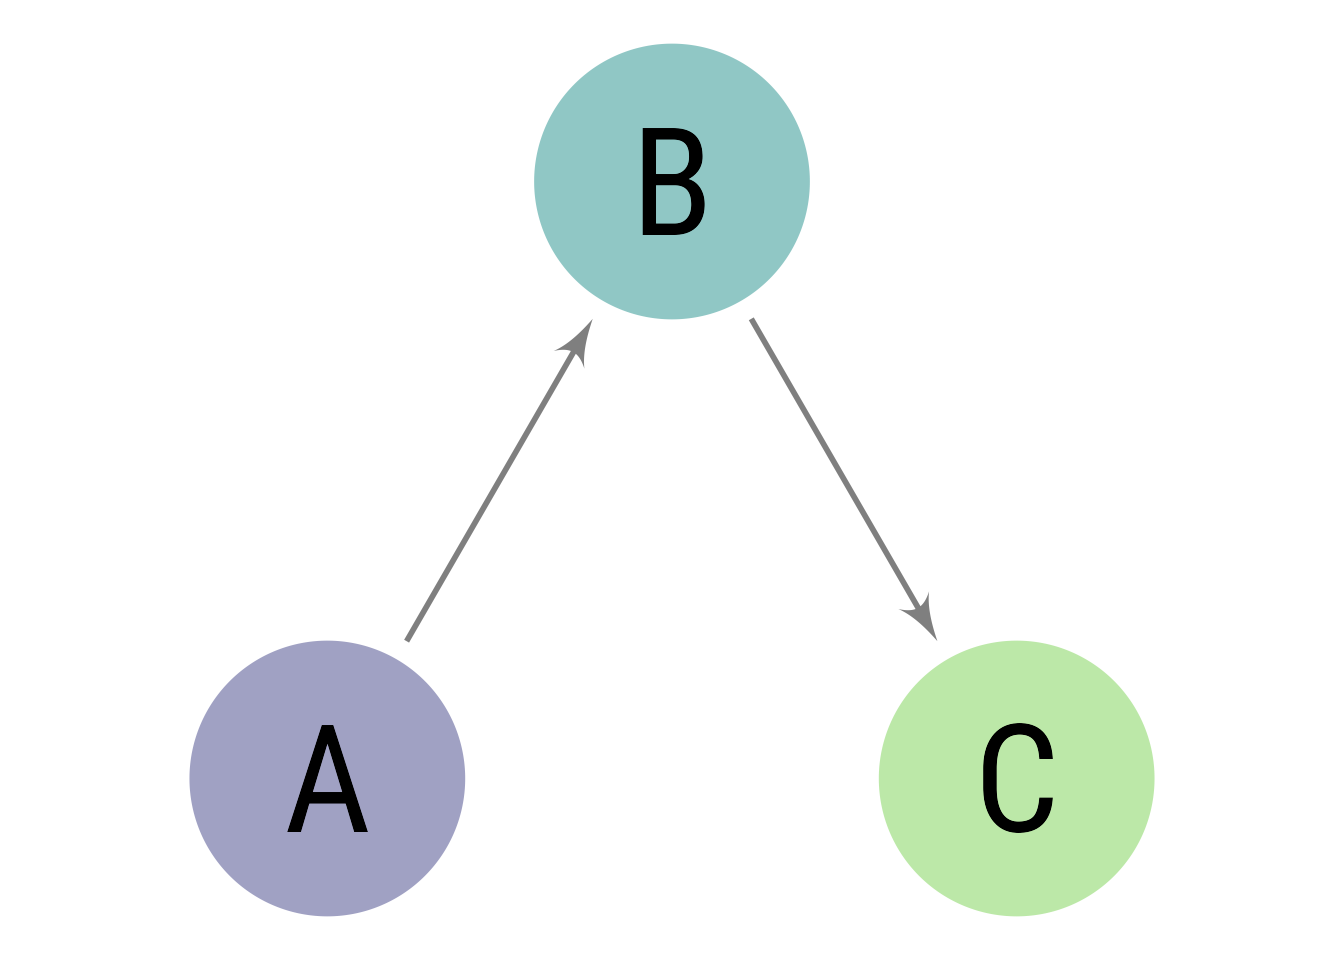
\includegraphics{sampleimage.png}

{\noindent \emph{Note.} A note below the figure}

\end{figure}






\end{document}
